\documentclass{llncs}
\usepackage[utf8]{inputenc}
\usepackage{verbatim}
\usepackage{multicol}
\usepackage{llncsdoc}
\usepackage{amsmath}
\usepackage{amsfonts}
\usepackage{amssymb}
\usepackage{graphicx}
\usepackage{lmodern}
\usepackage{calc}
\usepackage{enumitem}
\usepackage{algpseudocode}
\usepackage{algorithm}
\usepackage{algorithmicx}

\algsetblockdefx[IfContinue]{IfContinue}{IfContinue}
{0}{0pt}
[0]{}
[1]{\textbf{if} #1 \textbf{continue}}

\algrenewcommand\algorithmicrequire{%
  \makebox[\widthof{\textbf{Output:}}][l]{\textbf{Input:}}}
  
 \algrenewcommand\algorithmicensure{%
  \textbf{Output:}}

\usepackage{color}
\usepackage{gnuplottex}
\usepackage{subcaption}
\usepackage{microtype}
\usepackage[normalem]{ulem}
\captionsetup{compatibility=false}
\usepackage{tikz}
\usetikzlibrary{trees,automata,positioning}
\usepackage{booktabs}
\usepackage{gnuplottex}
\usepackage{xparse}
\usepackage{epstopdf}
% For scaling gnuplottex
\ExplSyntaxOn
\DeclareExpandableDocumentCommand{\convertlen}{ O{cm} m }
 {
  \dim_to_unit:nn { #2 } { 1 #1 } cm
 }
\ExplSyntaxOff

%% For lattice figure
% Set the overall layout of the tree
\tikzstyle{level 1}=[level distance=3.0cm, sibling distance=0.6cm]
\tikzstyle{level 2}=[level distance=3.5cm, sibling distance=0.6cm]
\tikzstyle{level 3}=[level distance=3.5cm, sibling distance=0.6cm]

% Define styles for bags and leafs
\tikzstyle{l1} = [rectangle, text width=5em, text centered]
\tikzstyle{l2} = [rectangle, text width=5em, text centered]
\tikzstyle{l3} = [rectangle, text width=5em, text centered]

% only when using asmthm
%\newtheorem{definition}{Definition}
%\newtheorem{theorem}{Theorem}

\author{Micky Faas \and Matthijs van Leeuwen}
\title{VOUW: Geometric Pattern Mining using the MDL Principle}
\institute{Leiden Institute for Advances Computer Science}
\begin{document}

\section{Introduction}

Frequent pattern mining \cite{fpmbook2014} is the well-known subfield of data mining that aims to find and extract recurring substructures from data, as a form of knowledge discovery. The generic concept of pattern mining has been instantiated for many different types of patterns, e.g., for item sets (in Boolean transaction data), subgraphs (in graphs/networks), and episodes (in sequences). So far, however, little research has been done on pattern mining for raster-based data, i.e., geometric matrices in which the row and column orders are fixed. The exception is geometric tiling \cite{gionis2004,tatti2012}, but that problem only considers tiles, i.e., rectangular-shaped patterns, in Boolean data.

In this paper we generalise this setting in two important ways. First, we consider geometric patterns \emph{of any shape} that are geometrically connected, i.e., it must be possible to reach any element from any other element in a pattern by only traversing elements in that pattern. Second, we consider \emph{discrete geometric data} with any number of possible values (which includes the Boolean case). We call the resulting problem \emph{geometric pattern mining}.

Figure~\ref{fig-example1} illustrates an example of geometric pattern mining.  Figure~\ref{fig-example1a} shows a $32 \times 24$ grayscale `geometric matrix', with each element in $[0,255]$, apparently filled with noise. If we take a closer look at all horizontal pairs of elements, however, we find that the pair $(146,11)$ is, amongst others, more prevalent than expected from `random noise' (Figure~\ref{fig-example1b}). If we would continue to try all combinations of elements that `stand out' from the background noise, we would eventually find four copies of the letter `I' set in 16 point Garamond Italic (Figure~\ref{fig-example1c}).

The 35 elements that make up a single `I' in the example form what we call a \emph{geometric pattern} that occurs four times. Since these occurrences jointly cover a substantial part of the matrix, we could use this pattern to describe the matrix more succinctly than by 768 unrelated values. That is, we could describe it as 628 unrelated values plus pattern `I' at locations $(5,4), (11,11), (20,3), (25,10)$, hereby separating structure from accidental (noise) data. Since the latter requires less space, we have compressed the data. At the same time we have learned something about the data, namely that it contains four I's. This suggests that we can use compression as a criterion to find patterns that describe the data.

\begin{figure}[t]
\centering
\begin{subfigure}[t]{0.35\textwidth}
\centering
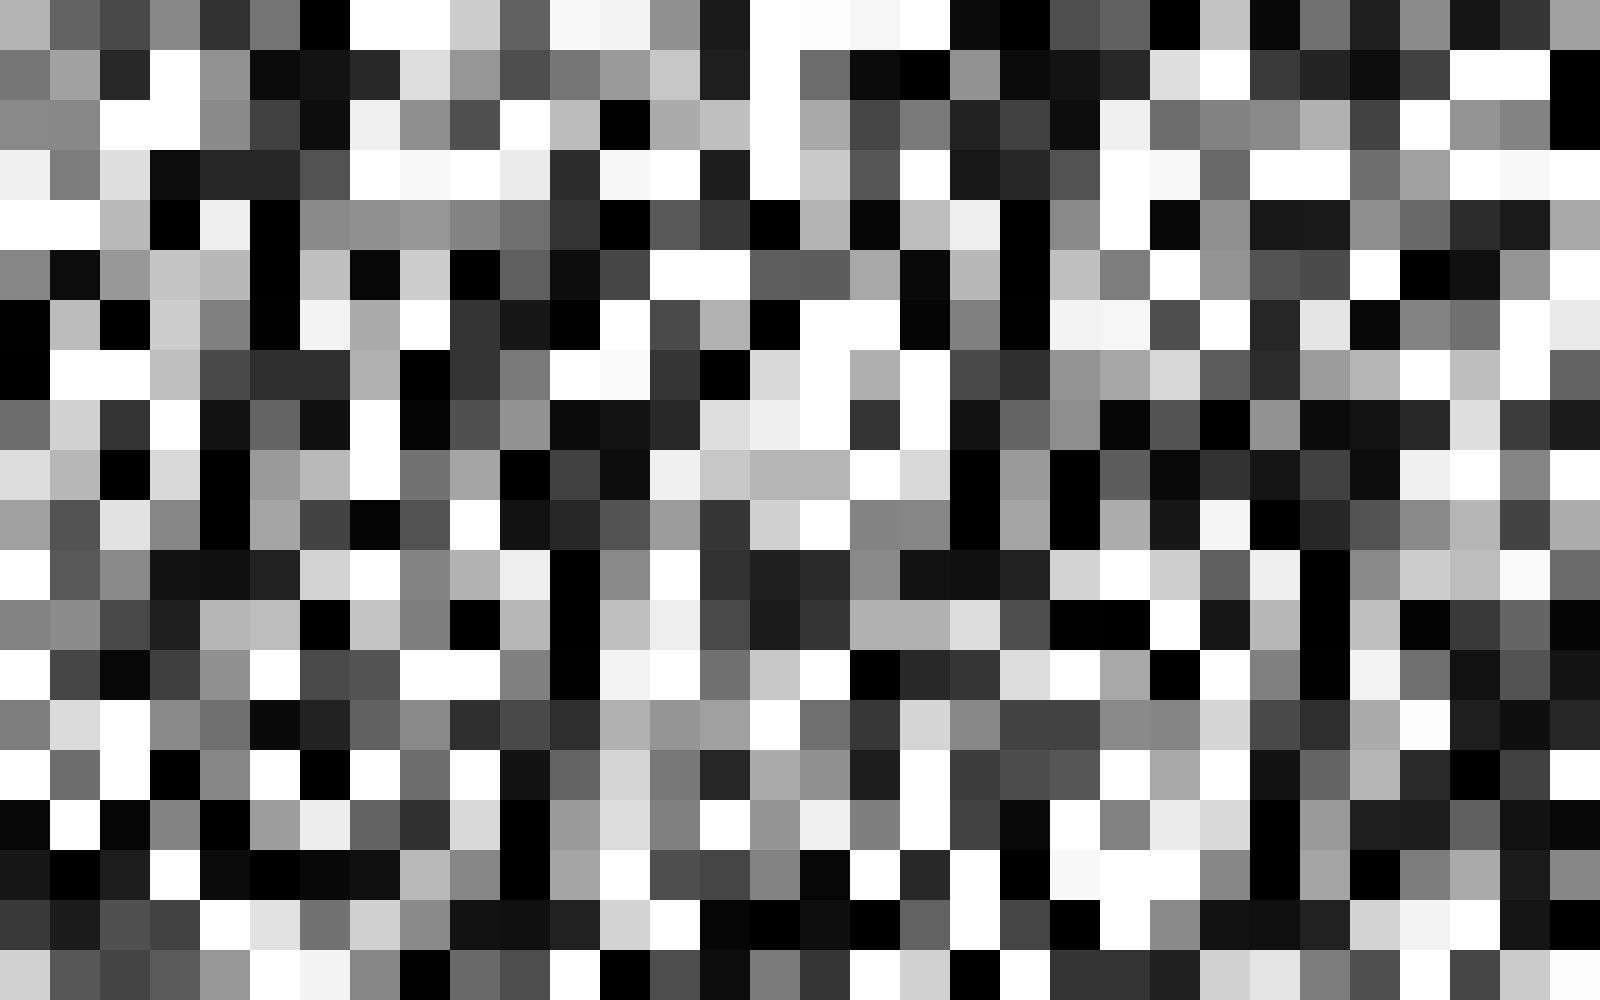
\includegraphics[scale=.25]{img/Garamond-I_cropped.png}
\caption{$32\times 24$ `geometric matrix'.}
\label{fig-example1a}
\end{subfigure}%
~
\begin{subfigure}[t]{0.20\textwidth}
\centering
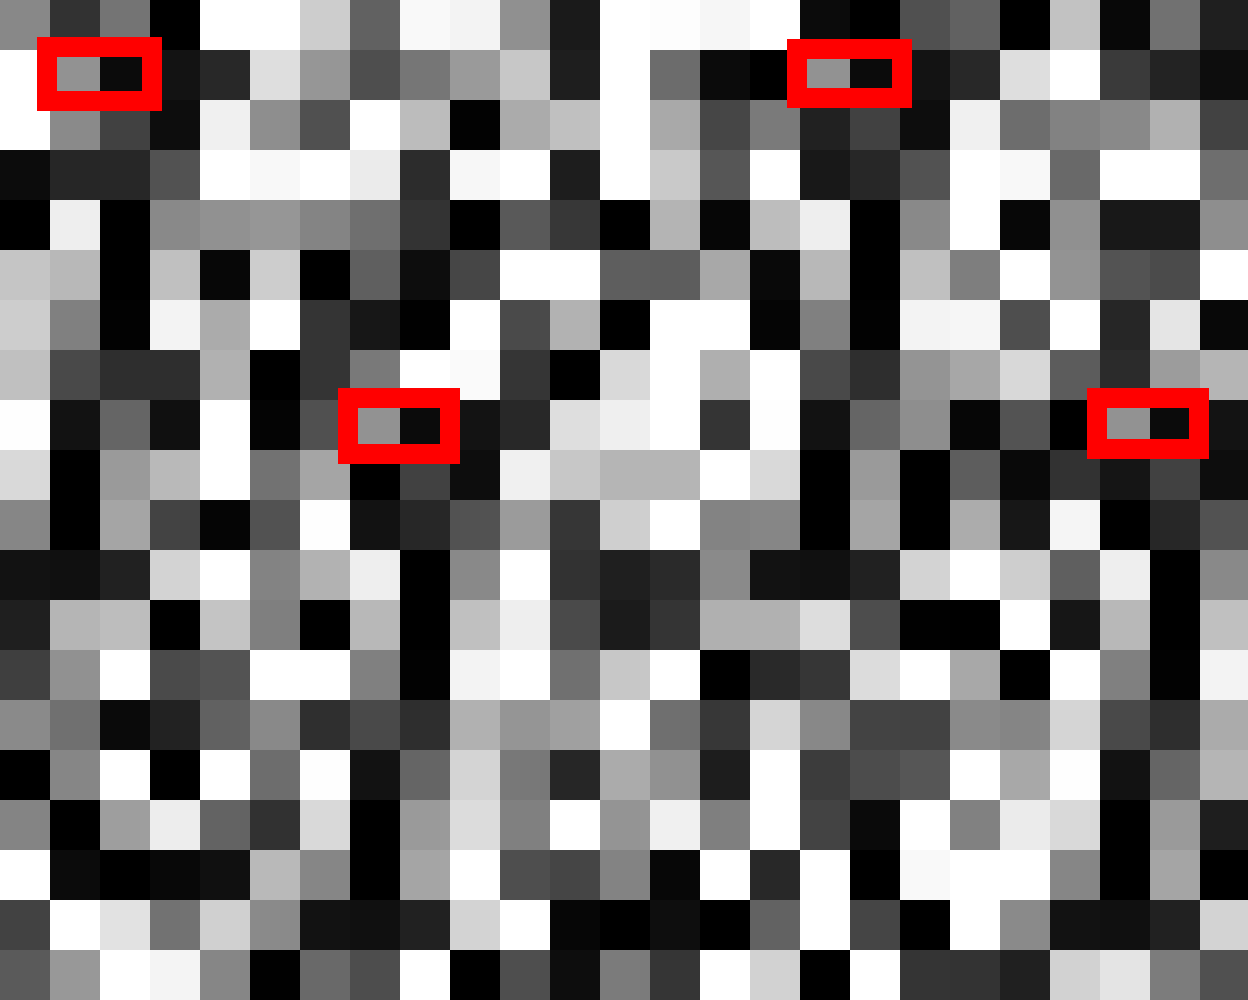
\includegraphics[scale=.25]{img/Garamond-I-highlight_cropped.png}
\caption{Pair $(146,11)$.}
\label{fig-example1b}
\end{subfigure}%
~
\begin{subfigure}[t]{0.37\textwidth}
\centering
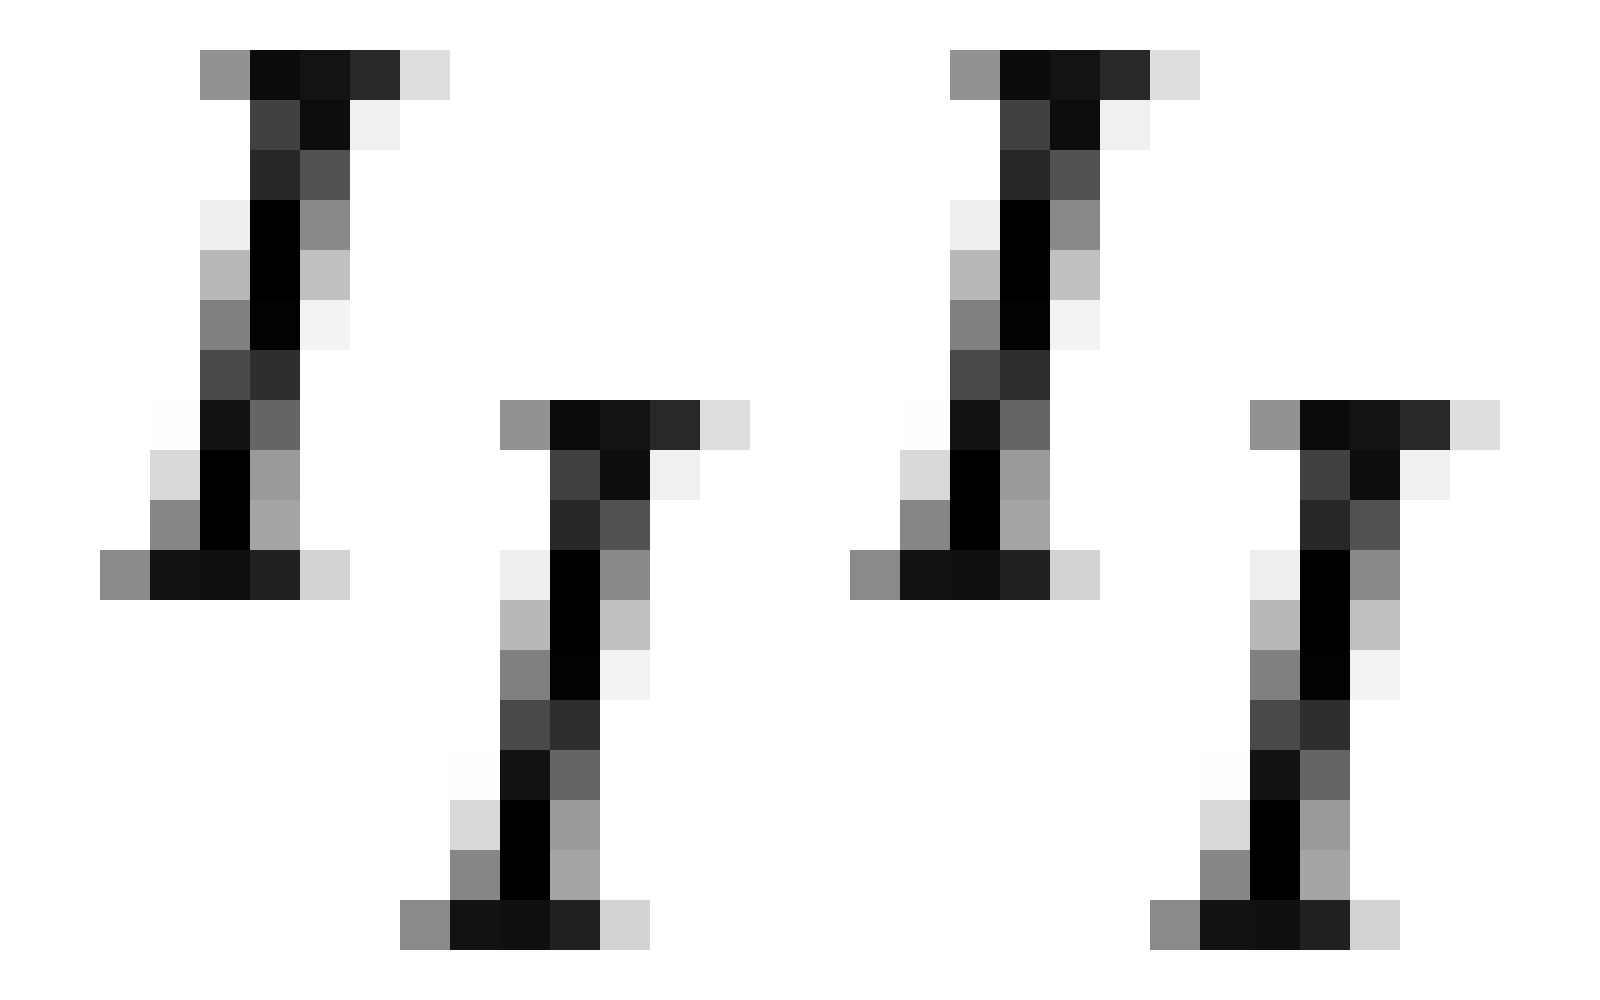
\includegraphics[scale=.25]{img/Garamond-I-clean_cropped.png}
\caption{Pattern `I' occurs four times.}
\label{fig-example1c}
\end{subfigure}%
\caption{Geometric pattern mining example. Each element is in $[0,255]$.}
\label{fig-example1}
\end{figure}  

\smallskip
\noindent \textbf{Approach and contributions}. Our first contribution is that we introduce and formally define \emph{geometric pattern mining}, i.e., the problem of finding recurring local structure in geometric, discrete matrices. Although we restrict the scope of this paper to two-dimensional data, the generic concept applies to larger number of dimensions. Potential applications include the analysis of satellite imagery, texture recognition, and clustering.

We distinguish three subtypes of geometric patterns. The first concerns the discovery of \emph{exactly identical} patterns; the second concerns \emph{fault-tolerant} patterns, which can have noisy occurrences; the third concerns \emph{transformational} patterns, which are identical after some transformation (such as mirror, inverse, rotate, etc.). Each consecutive subtype makes the problem more expressive and hence more complex. Further, we distinguish the discovery of patterns from either an otherwise empty matrix, differently distributed noise, or similarly distributed noise, again in order of increasing difficulty.

As many geometric patterns can be found in a typical matrix, it is crucial to find a compact set of patterns that together describes the structure in the data well. We regard this as a model selection problem, where a model is defined by a set of patterns. Following our observation above, that geometric patterns can be used to compress the data, our second contribution is the formalisation of the model selection problem by using the \emph{Minimum Description Length (MDL) principle} \cite{rissanenmdl,grunwaldmdl}. Central to MDL is the notion that `learning' can be thought of as `finding regularity' and that regularity itself is a property of data that is exploited by \emph{compressing} said data. This matches very well with the goals of pattern mining, as a result of which the MDL principle has proven very successful for MDL-based pattern mining \cite{krimp,classy}.

Finally, our third contribution is VOUW, a heuristic algorithm for MDL-based geometric pattern mining that (1) finds compact yet descriptive sets of patterns, (2) requires no parameters, and (3) is tolerant to noise in the data. We empirically evaluate VOUW on synthetic data and demonstrate that it is able to accurately recover planted patterns.

\end{document}
